\part{Results}
\label{pa:results}
\chapter{Graph analysis}
PPI network from irefweb.
downloaded with these settings: %picture from irefweb
irefweb said 109276 interactions 
after hgnc it was 43706 (perturbation: 60\% from iref)
after clustering it was 13183 (perturbation: 87,9\% from iref - 69,8\% from hgnc) % not used
only uniprot and refseq
uniprot said
\section{Creating a network}
Converting from proteins to genes through HGNC data resulten in a 60\% data
network edge perturbation. From 100k ish links to 40k ish.
\subsection{Creating connections}
\subsection{Adding weights}
\section{Ranking results}
Talking about \gls{mcl} results
\begin{table}[H]
    \centering
    \begin{tabular}{| l | c | c | c | c | c | c |}
        \hline
        \textbf{Inflation} & \textbf{Clusters} & \textbf{Avg.  cluster size} &
        \textbf{Max. cluster size} & \textbf{Min. cluster size} &
        \textbf{Modularity} \\
        \hline
        1.6 & 1068 & 8.88 & 968 & 2 & 0.367 \\
        1.8 & 1400 & 6.60 & 660 & 2 & 0.307 \\
        2.0 & 1599 & 5.68 & 405 & 2 & 0.269 \\
        2.5 & 2053 & 4.20 & 179 & 2 & 0.223 \\
        3.0 & 2210 & 3.75 & 122 & 2 & 0.199 \\
        \hline
    \end{tabular}
    \caption{MCL clustering parameter and statistic results}
    \label{tab:mcl-inflation}
\end{table}
The modularity of the clustered networks gives an indicator of how well the
process of creating the clusters went. Modularity is given as a score from 0 to
1. A score closer to 1 is more preferrable, as this indicates that the clusters
created have a good degree of separation to the other clusters in the network.
The preferred score to end up with would be around 0.8, but in this network
there has been a good amount of perturbation through the protein-to-gene
process. Modularity is not the only indicator of how well a network was
clustered, hence the choice of not setting the inflation value in \gls{mcl} to
1.6, but rather 1.8. When a lower inflation value is set, \gls{mcl} does not
separate edges between nodes as vigorously and as a direct cause, inflation will
go up. Taking the other attributes in the table \ref{tab:mcl-inflation} into
consideration, 1.8 seemed like the best inflation value. An inflation value of
1.8 has also been proved to be good for large high-throughput constructed
protein-protein networks with a large amount of alterations\cite{mcl-inflation}.
%% Move this part to methods?

\section{Cross-validation}
Executing a cross-validation on the iRefWeb with PRWP and MAA rankings had two
purposes. The first being to prove the fact that every gene that had its prior
score removed by the cross-validation, should be found in the results of the
cluster ranking and identified as candidate biomarkers. 

The second purpose was to analyze the distribution of the genes with prior
scores removed by the cross-validation in terms of how they placed in the
cluster ranking. The analysis of this distribution was done by dividing the
amount of genes removed by cross-validation in a cluster by the total amount of
genes in the same cluster. This operation was repeated for every cluster in the
ranking, resulting in a distribution of the average amount of genes removed by
cross-validation, that was detected by Ranklust together with post-processing of
data, as cancer candidate biomarkers. A distinct descending distribution from
high to low ranked clusters would indicate that most of the genes, with a prior
score of their relevance to prostate cancer, was ranked in a way that achieved
the goal of Ranklust; ranking clusters in biological network according to
network structure and prior knowledge of relevance to diseases.

\subsection{Cross-validation in PRWP}
\hspace*{-1cm}\begin{figure}[H]
    \label{fig:irefweb-prwp}
    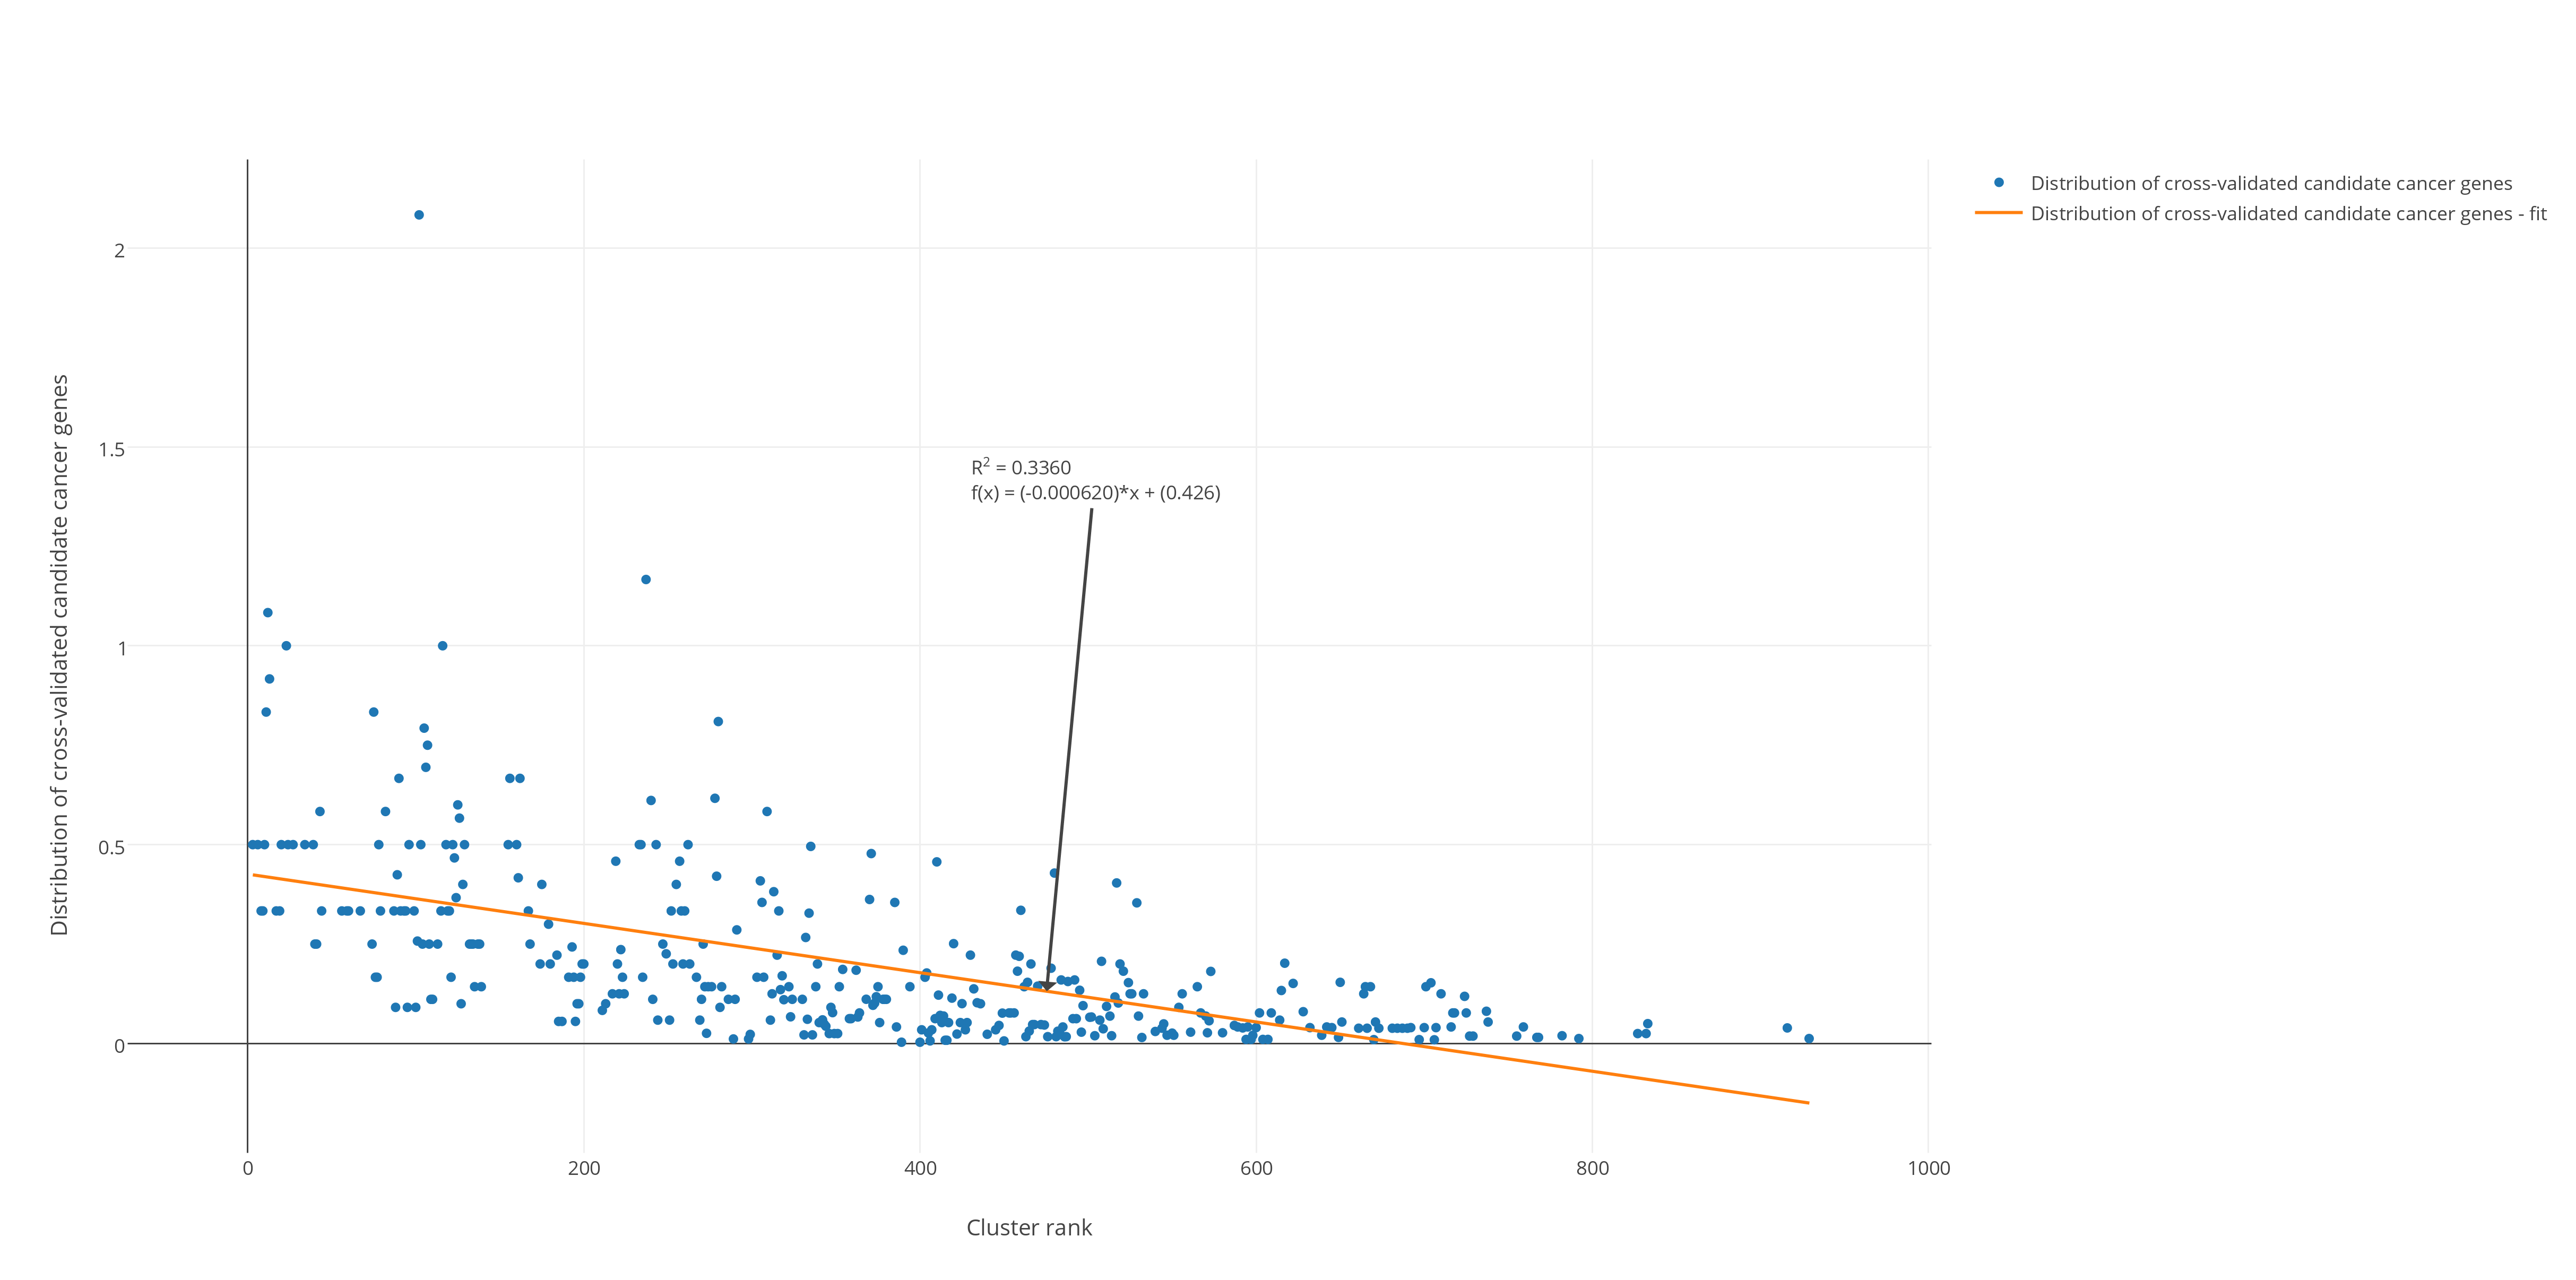
\includegraphics[scale=0.6]{cv_dist_total_filtered_prwp}
    \caption{Cross-validation distribution in clusters (PRWP)}
\end{figure}
This plot \ref{fig:irefweb-prwp} is developed from the 10 random
cross-validation runs ranked with PRWP. The results from this cross-validation
shows that the higher the rank of the cluster, the more candidate cancer genes
the cluster had.

\subsection{Cross-validation in MAA}
\hspace*{-1cm}\begin{figure}[H]
    \label{fig:irefweb-maa}
    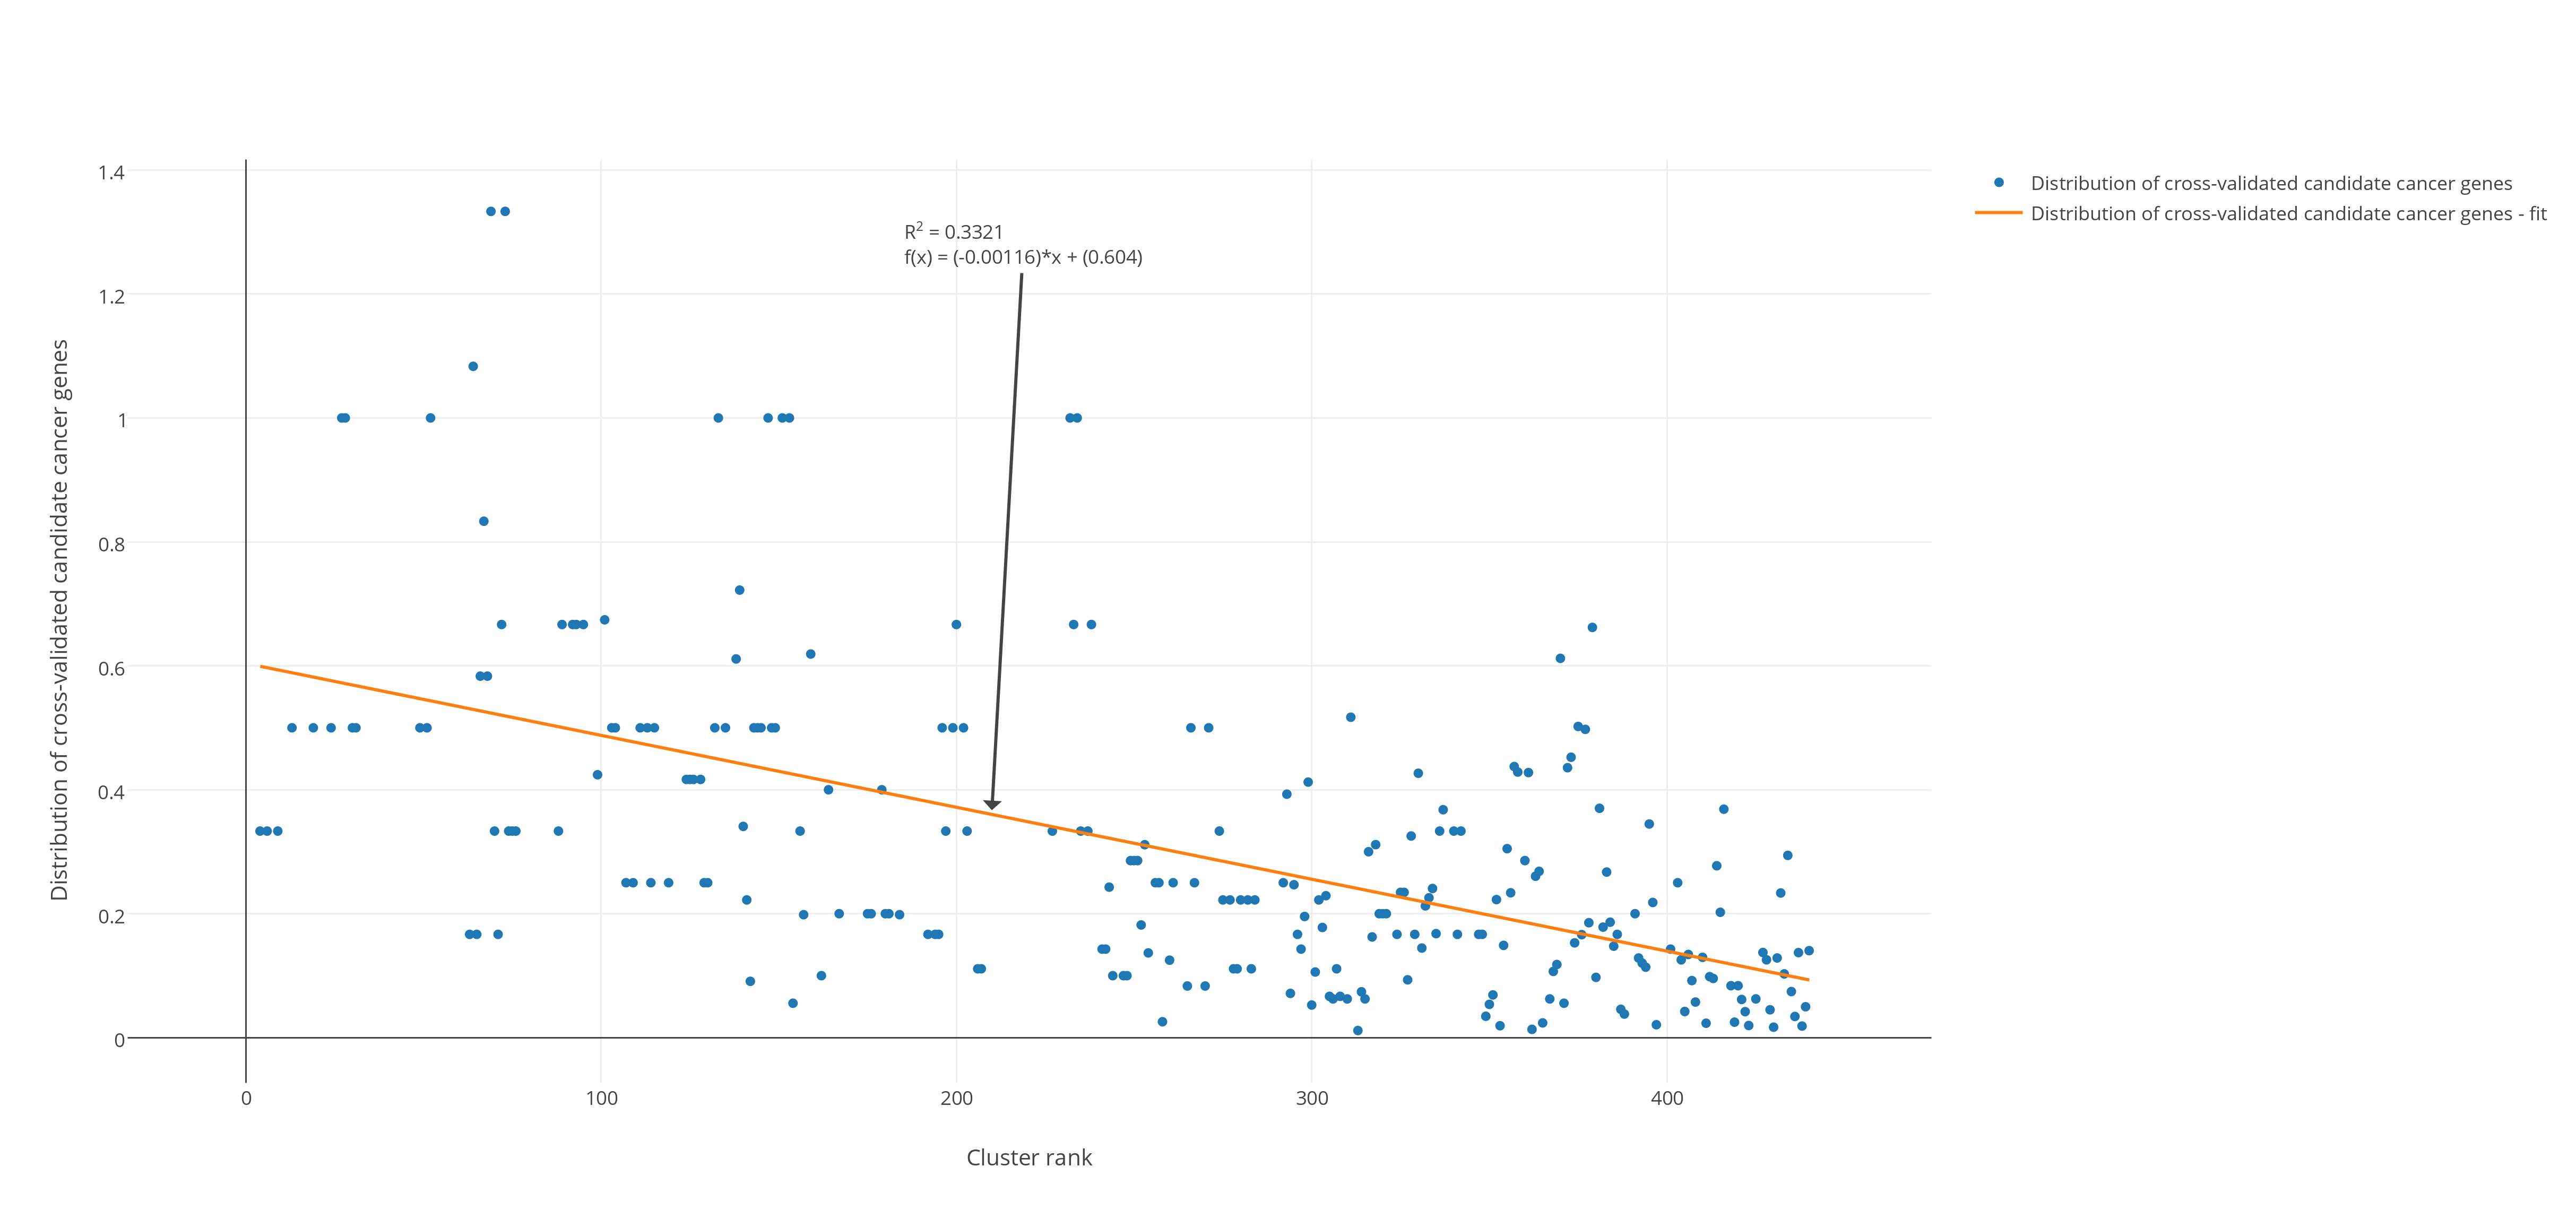
\includegraphics[scale=0.6]{cv_dist_total_filtered_maa}
    \caption{Cross-validation distribution in clusters (MAA)}
\end{figure}
This plot \ref{fig:irefweb-maa} is developed from the 10 random
cross-validatioon runs ranked with MAA. The results from this cross-validation
shows that the higher the rank of the cluster, the more candidate cancer genes
the cluster had.

\subsection{PRWP versus MAA}
There is clearly a trend in both \gls{prwp} and \gls{maa}. The difference
between them being mainly the amount of clusters found and the coupling of
values around the linear regression fit. It is important to point out that this
is just a result over the distribution of candidate cancer genes at certain
ranks. Where the clusters resides in the rankings may be very different between
the \gls{prwp}} and \gls{maa}.

The fact that both of the ranking algorithms managed to get a descending amount
of prostate candidate cancer genes in the clusters, which was cross-validated
from the same \gls{golden} priors, indicates that a certain similarity of what
was mentioned in the previous paragraph. The similarity implicated here is how
different the ranking of the clusters are between \gls{prwp} and \gls{maa}.

The values in \gls{prwp} have a tighter coupling, in other words, the distance
the coordinates have in the scatter plot deviate less from the fit than the ones
in the \gls{maa} plot. The difference is not huge, as the coefficient of
determination indicates, 0.336 in \gls{prwp} against 0.332 in \gls{maa}. Both
ranking algorithms achieves a descending distribution of cross-validated genes
from the topmost to the lowest ranked cluster. But when comparing the
cross-validation results between \gls{prwp} and \gls{maa}, \gls{prwp} comes out
ahead by a margin in \gls{rsquared} value.

\section{Benchmarks}

% prwp
\subsection{Text mined and scored with z-values}
\begin{figure}[H]
    \label{fig:txt-iref-prwp}
    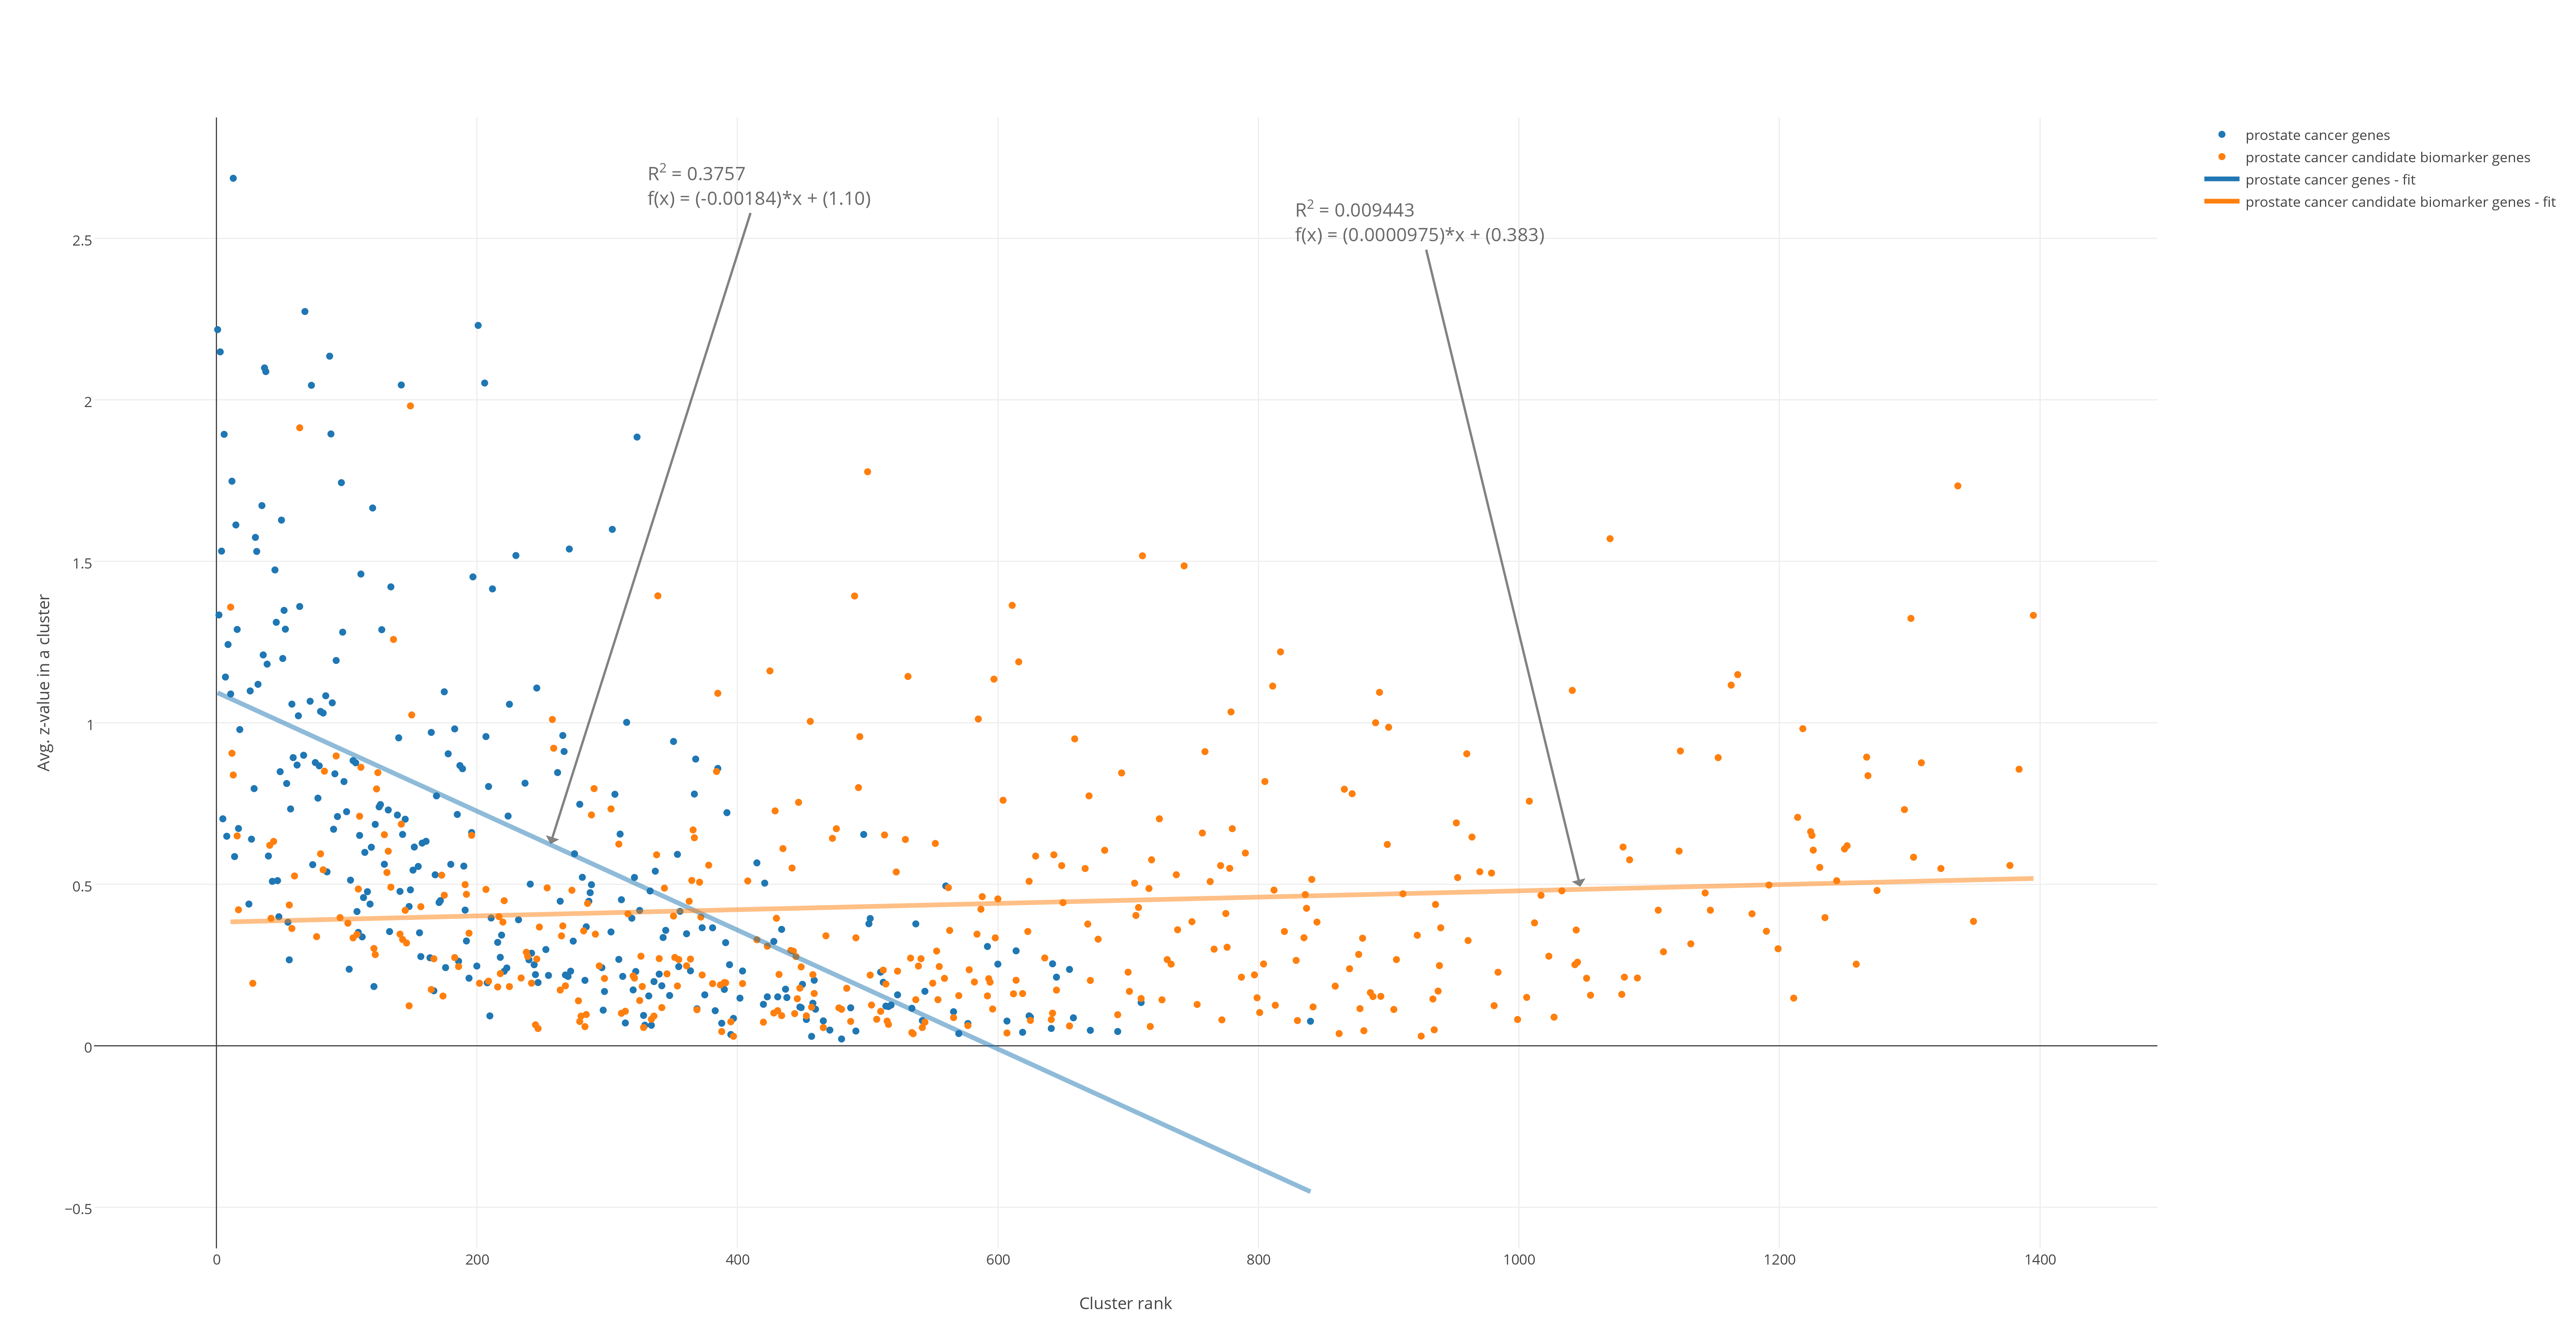
\includegraphics[width=15cm]{prwp_textmined_split}
    \caption{Average distribution of z-scores in clusters ranked by PRWP.}
\end{figure}
\begin{figure}[H]
    \label{fig:txt-iref-maa}
    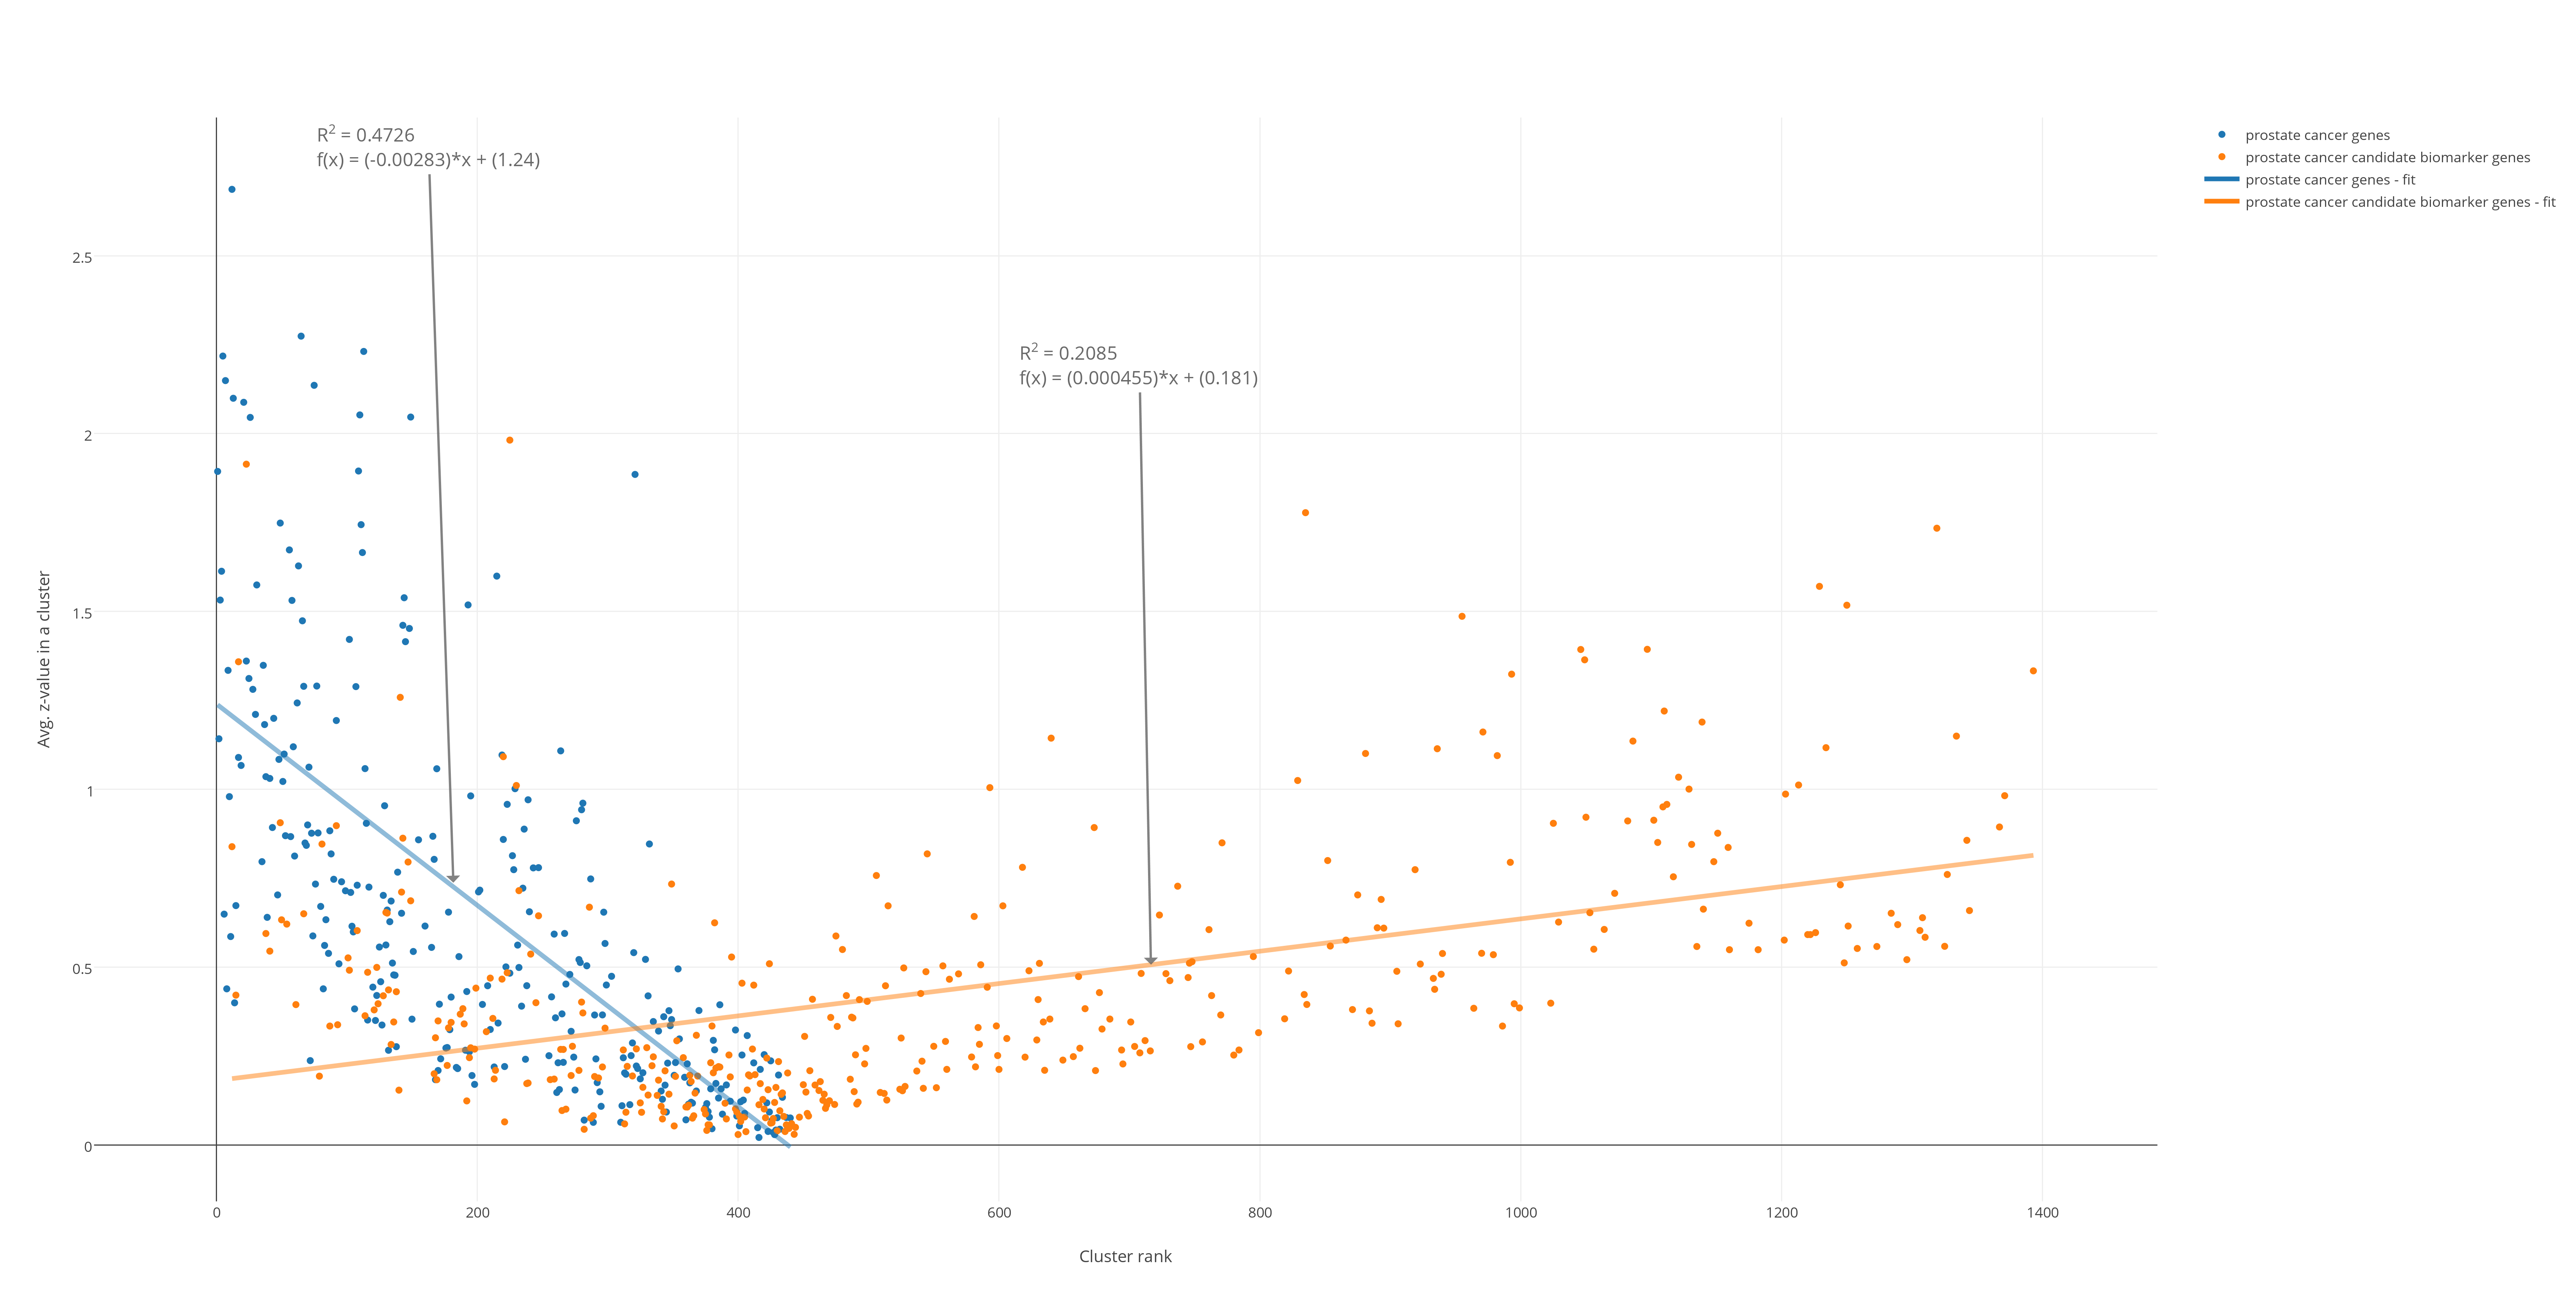
\includegraphics[width=15cm]{maa_textmined_split}
    \caption{Average distribution of z-scores in clusters ranked by MAA.}
\end{figure}

\subsection{Knowledge curated distribution of genes}
\begin{figure}[H]
    \label{fig:know-iref-prwp}
    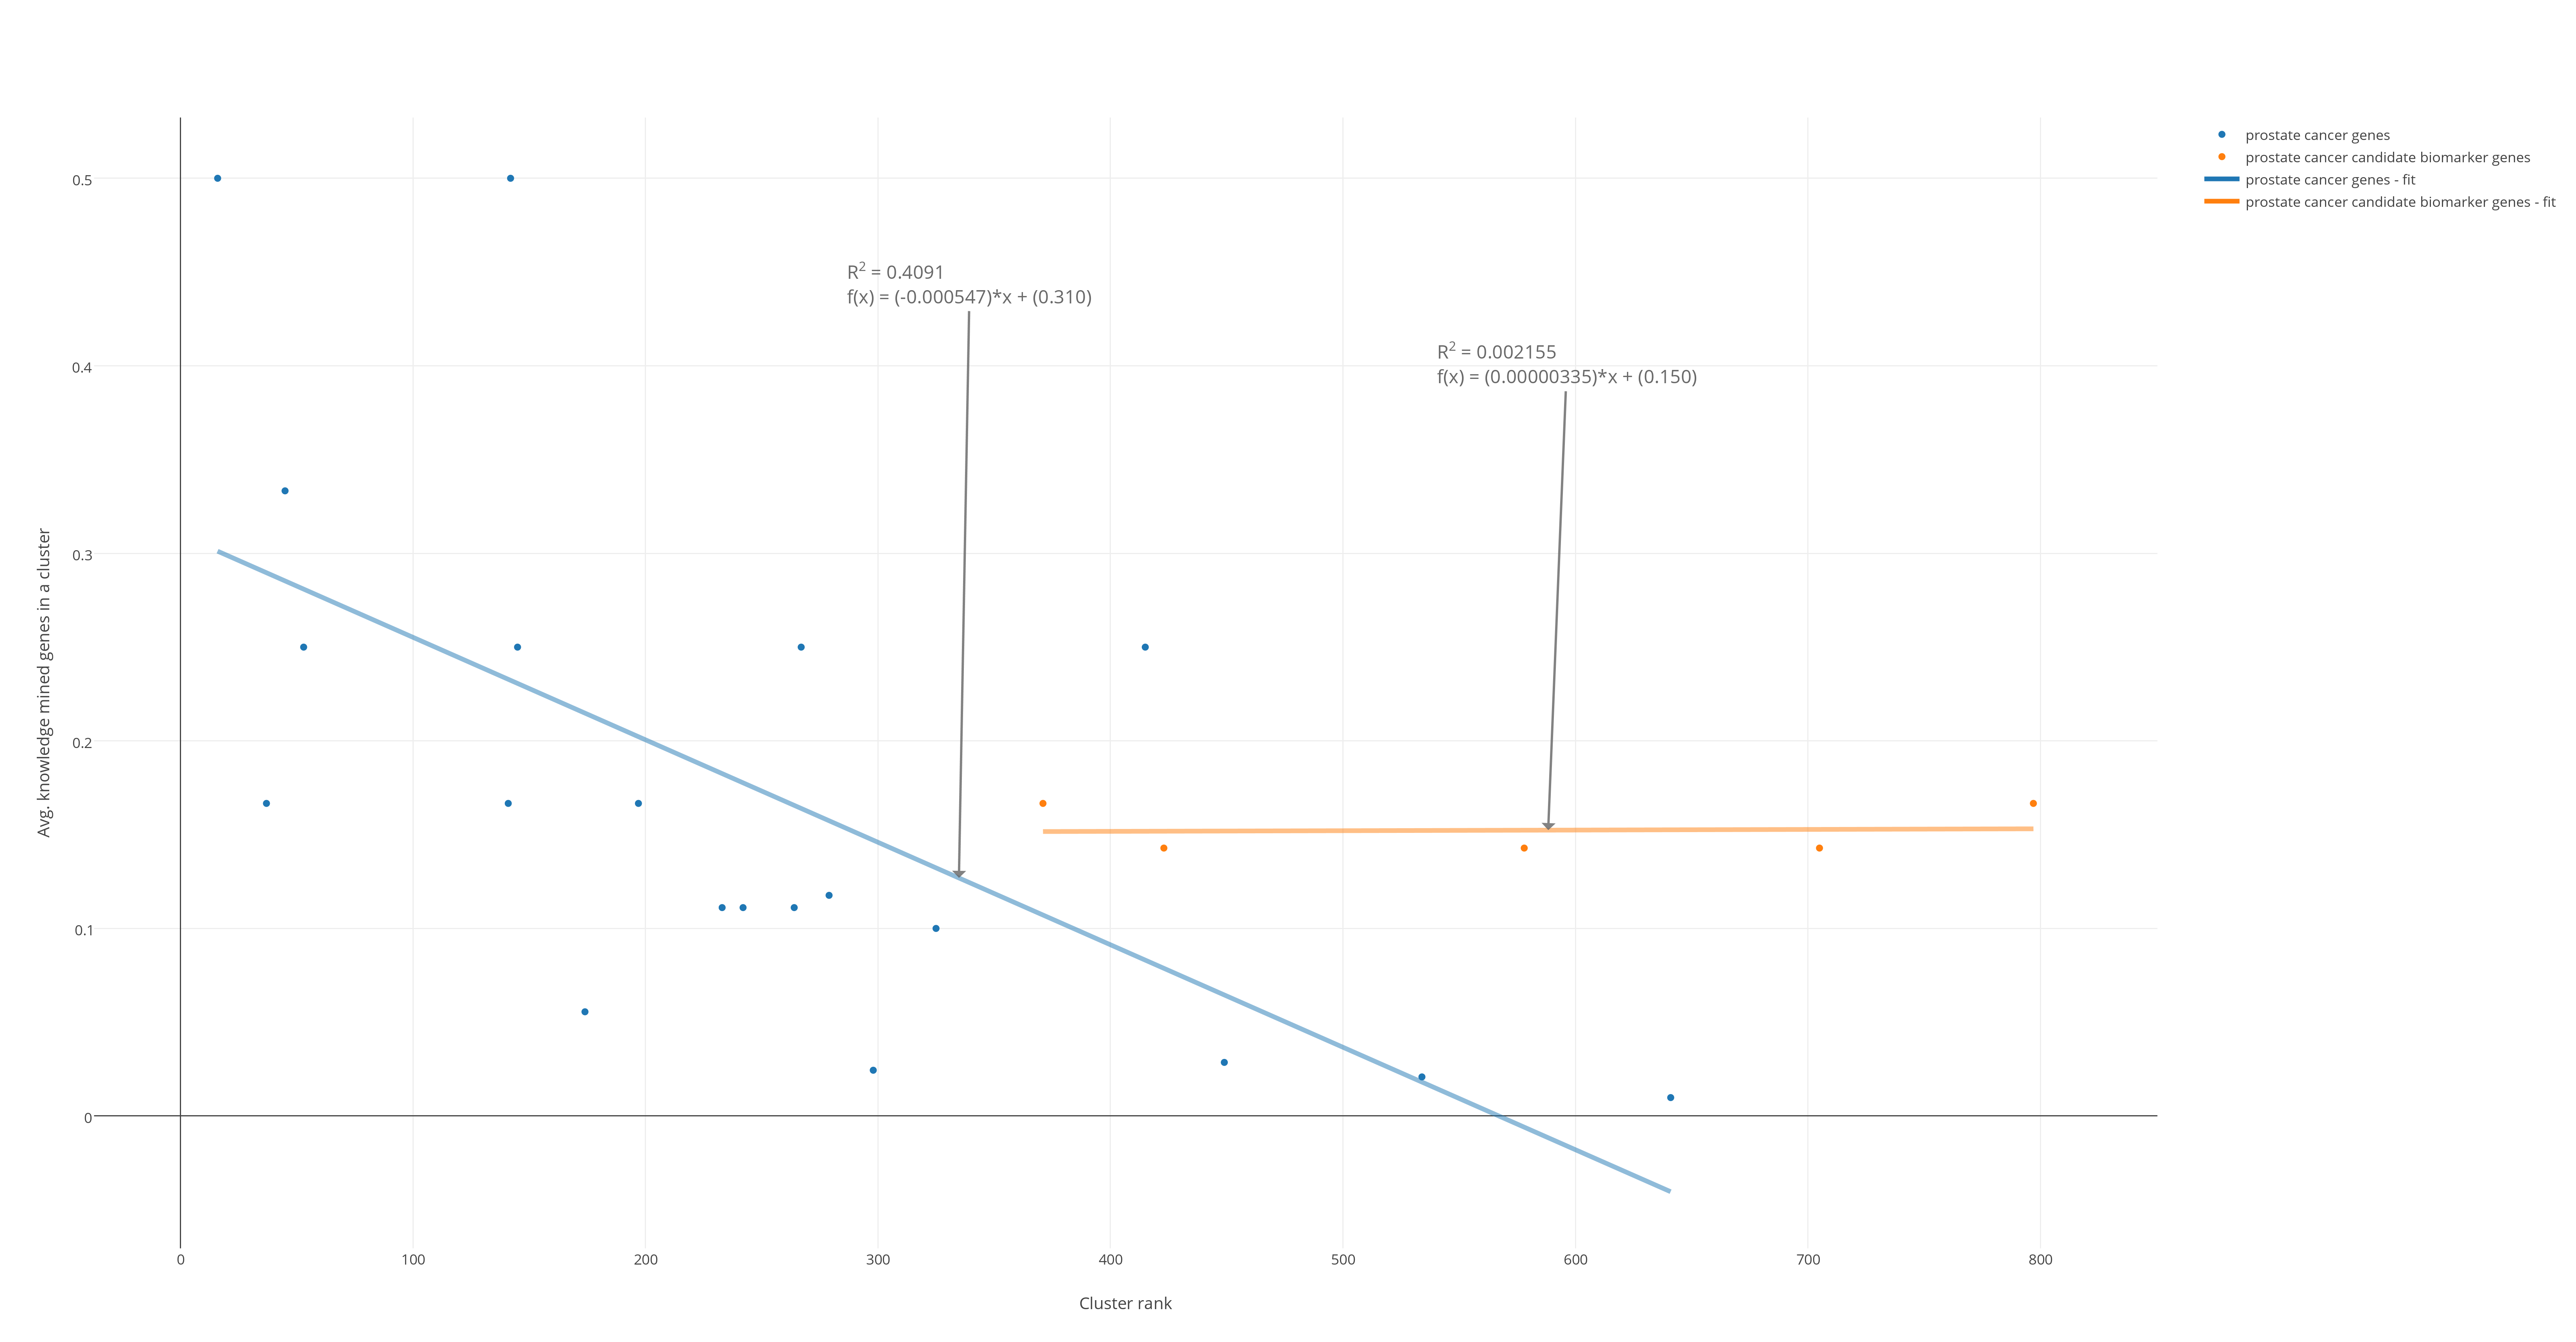
\includegraphics[width=15cm]{prwp_knowledge_split}
    \caption{Average distribution of curated knowledge mined genes in clusters
    ranked by PRWP.}
\end{figure}
\begin{figure}[H]
    \label{fig:know-iref-maa}
    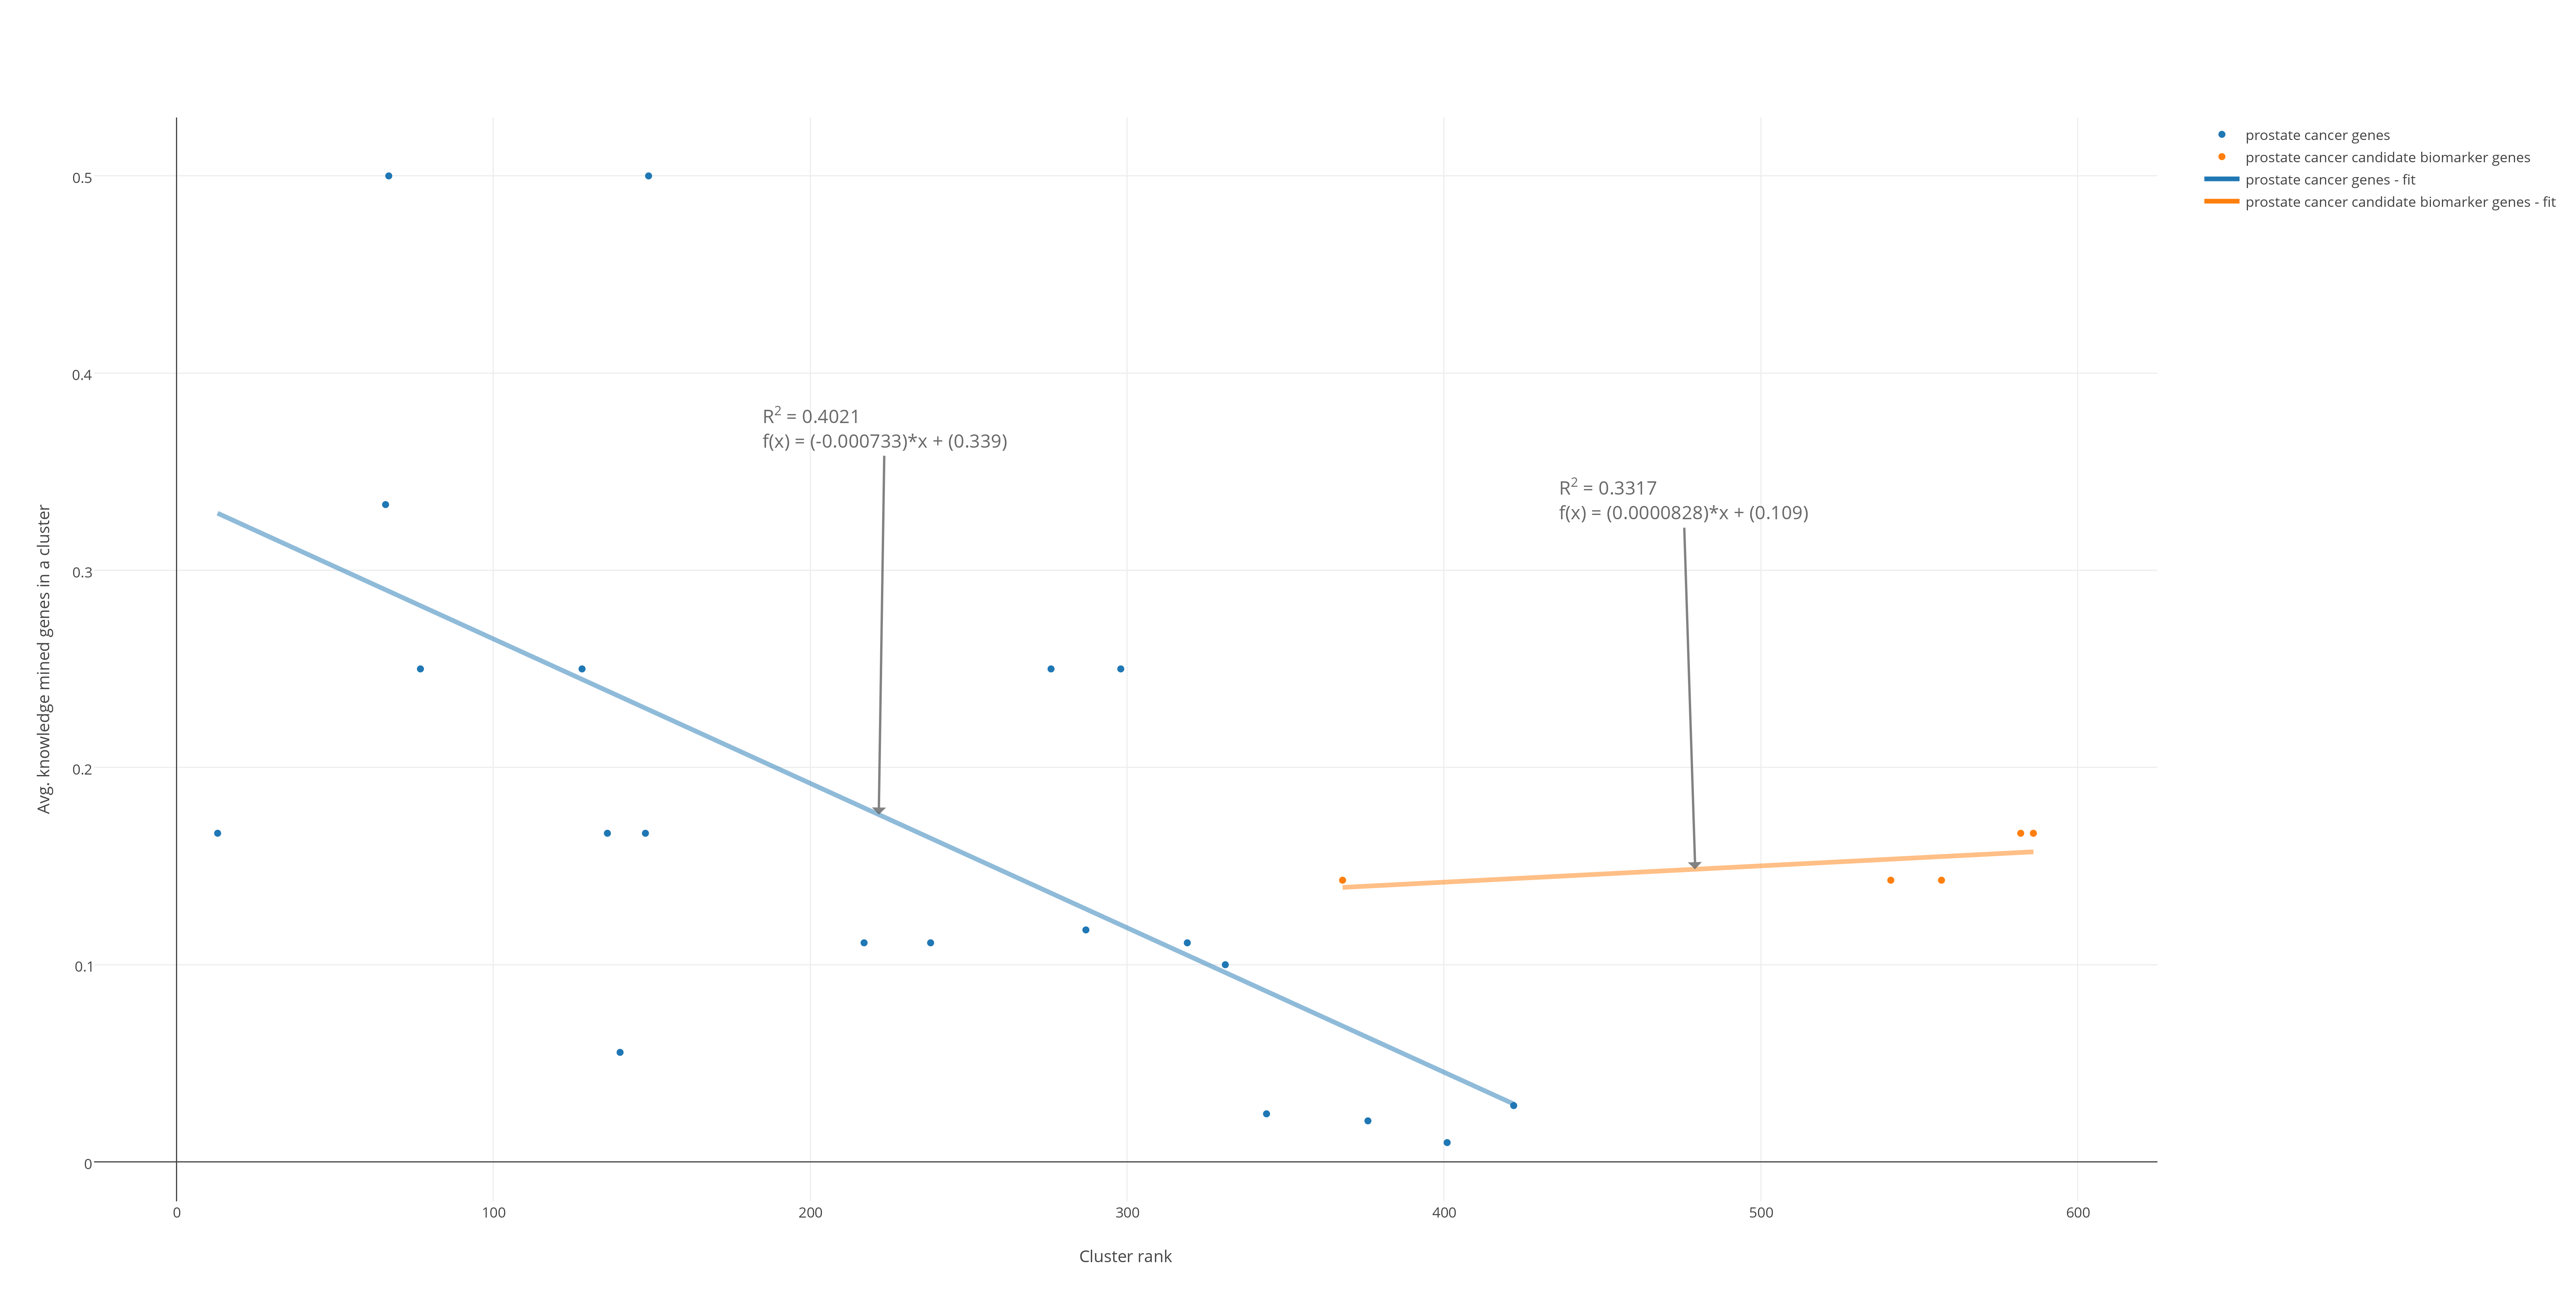
\includegraphics[width=15cm]{maa_knowledge_split}
    \caption{Average distribution of curated knowledge mined genes in clusters
    ranked by MAA.}
\end{figure}
\subsection{Experimental mined genes distribution of p-values in genes}
\begin{figure}[H]
    \label{fig:exp-iref-prwp}
    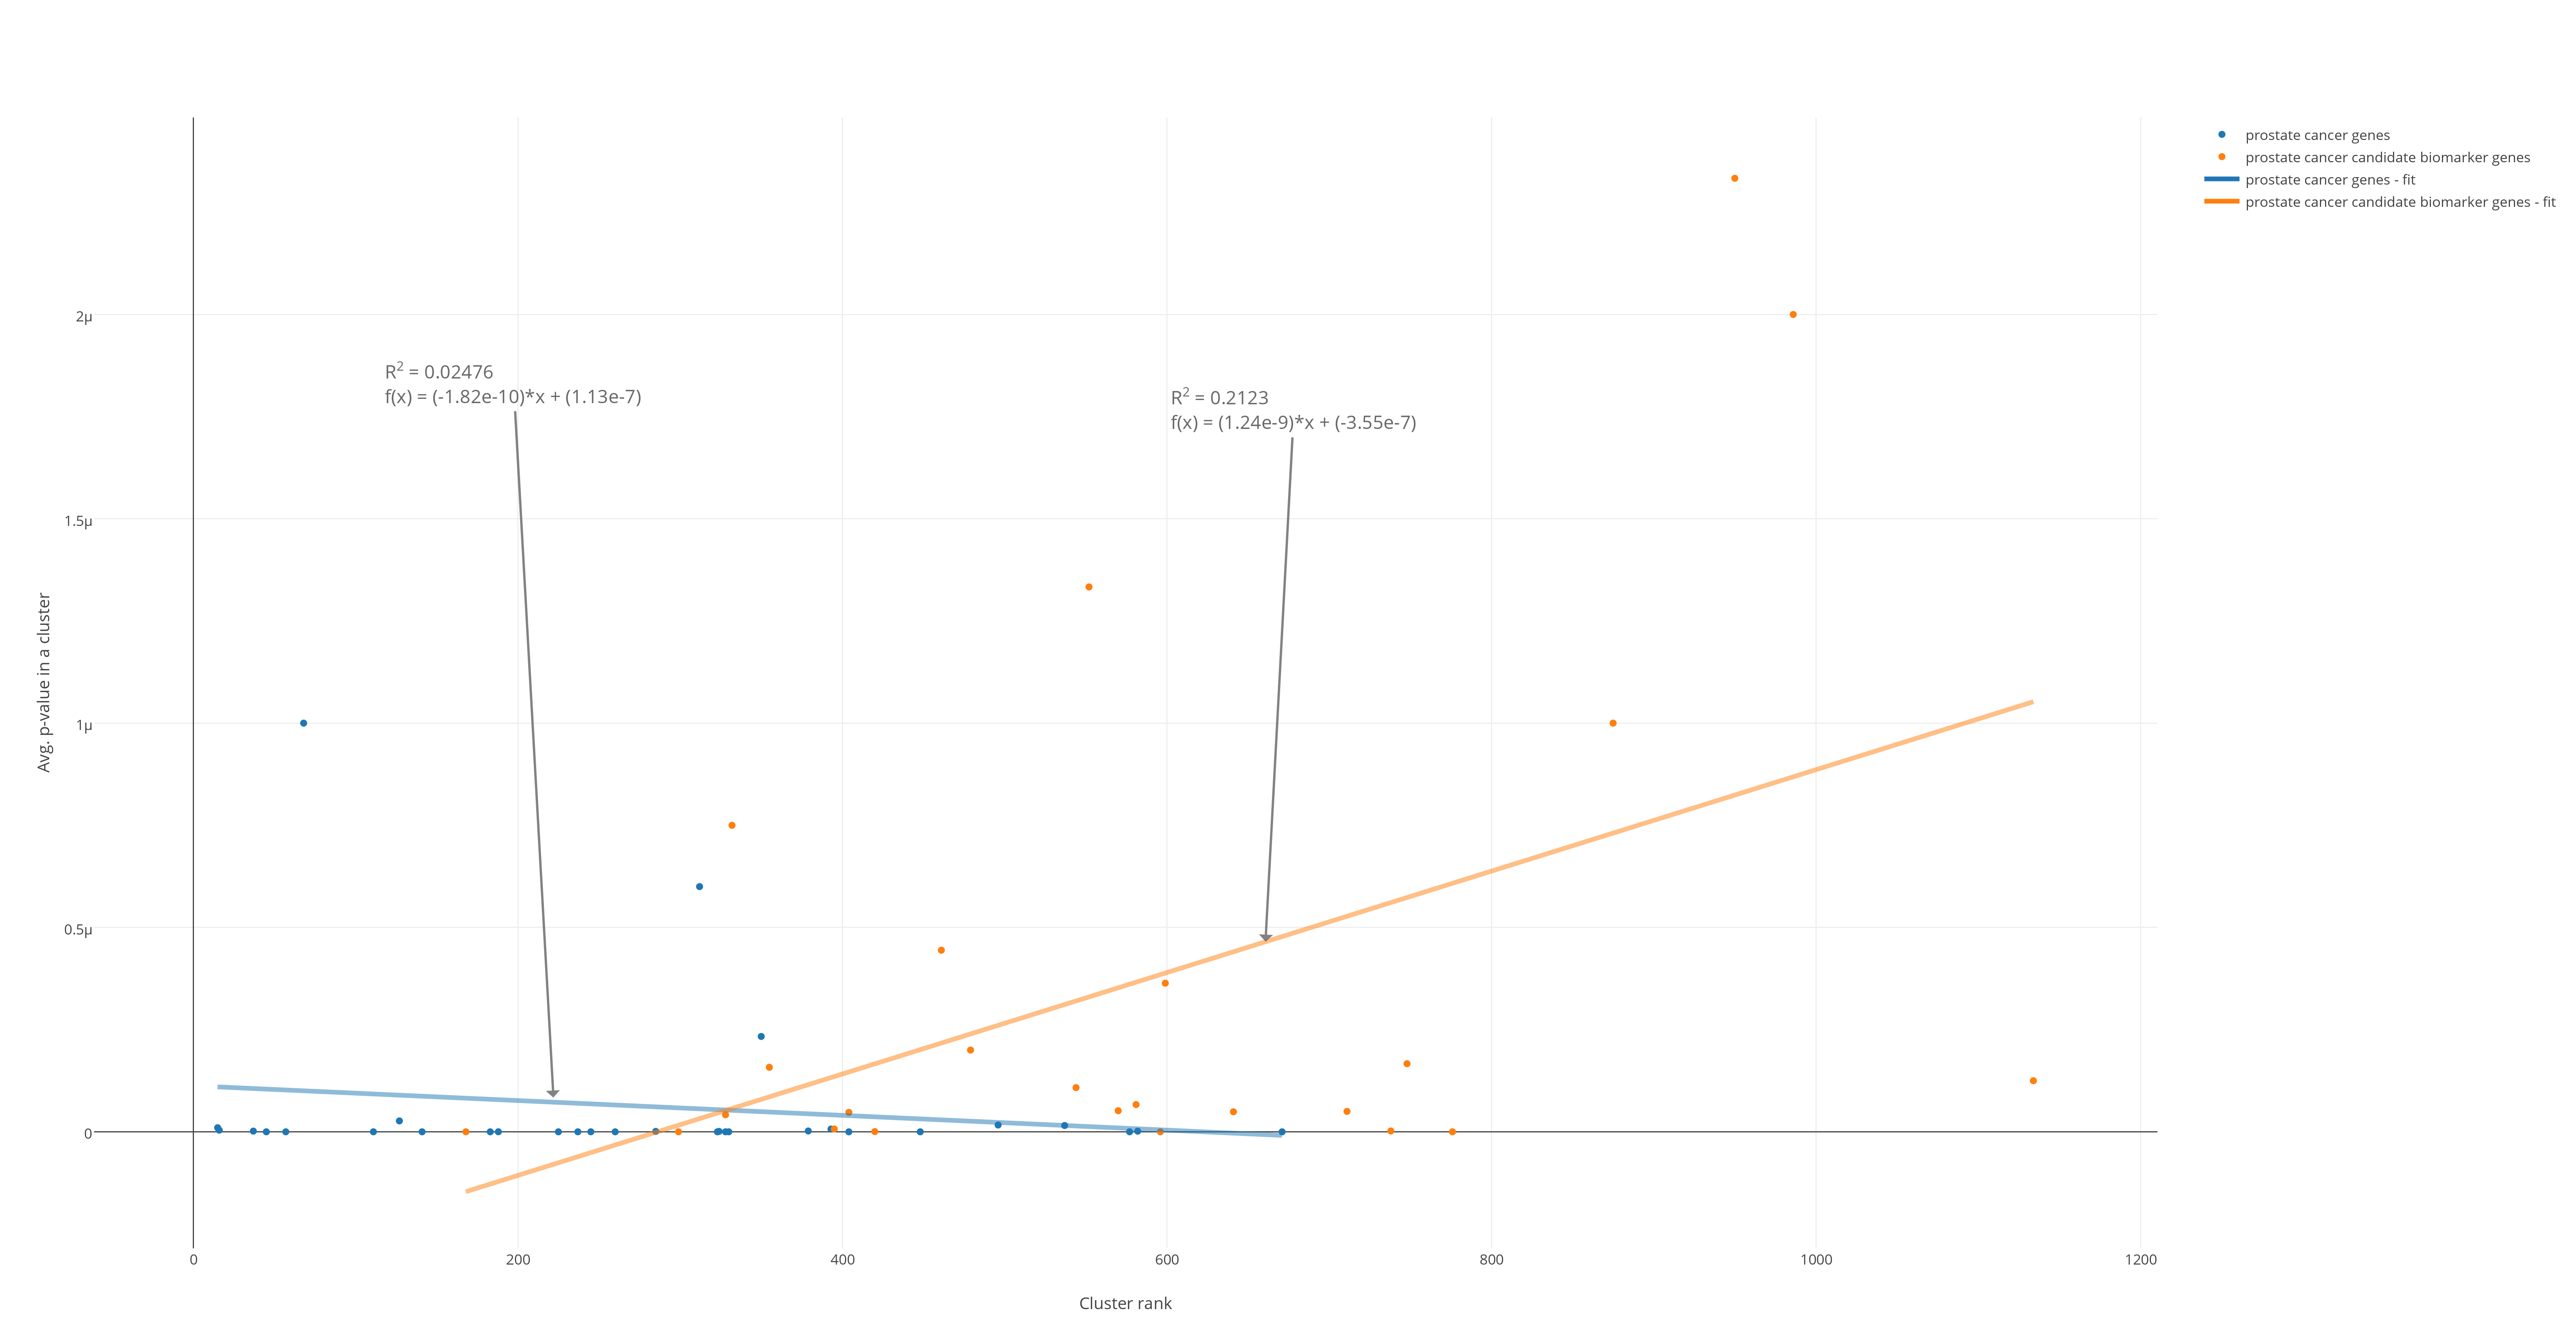
\includegraphics[width=15cm]{prwp_experimental_split}
    \caption{Average distribution of p-values in clusters ranked by PRWP.}
\end{figure}
\begin{figure}[H]
    \label{fig:exp-iref-maa}
    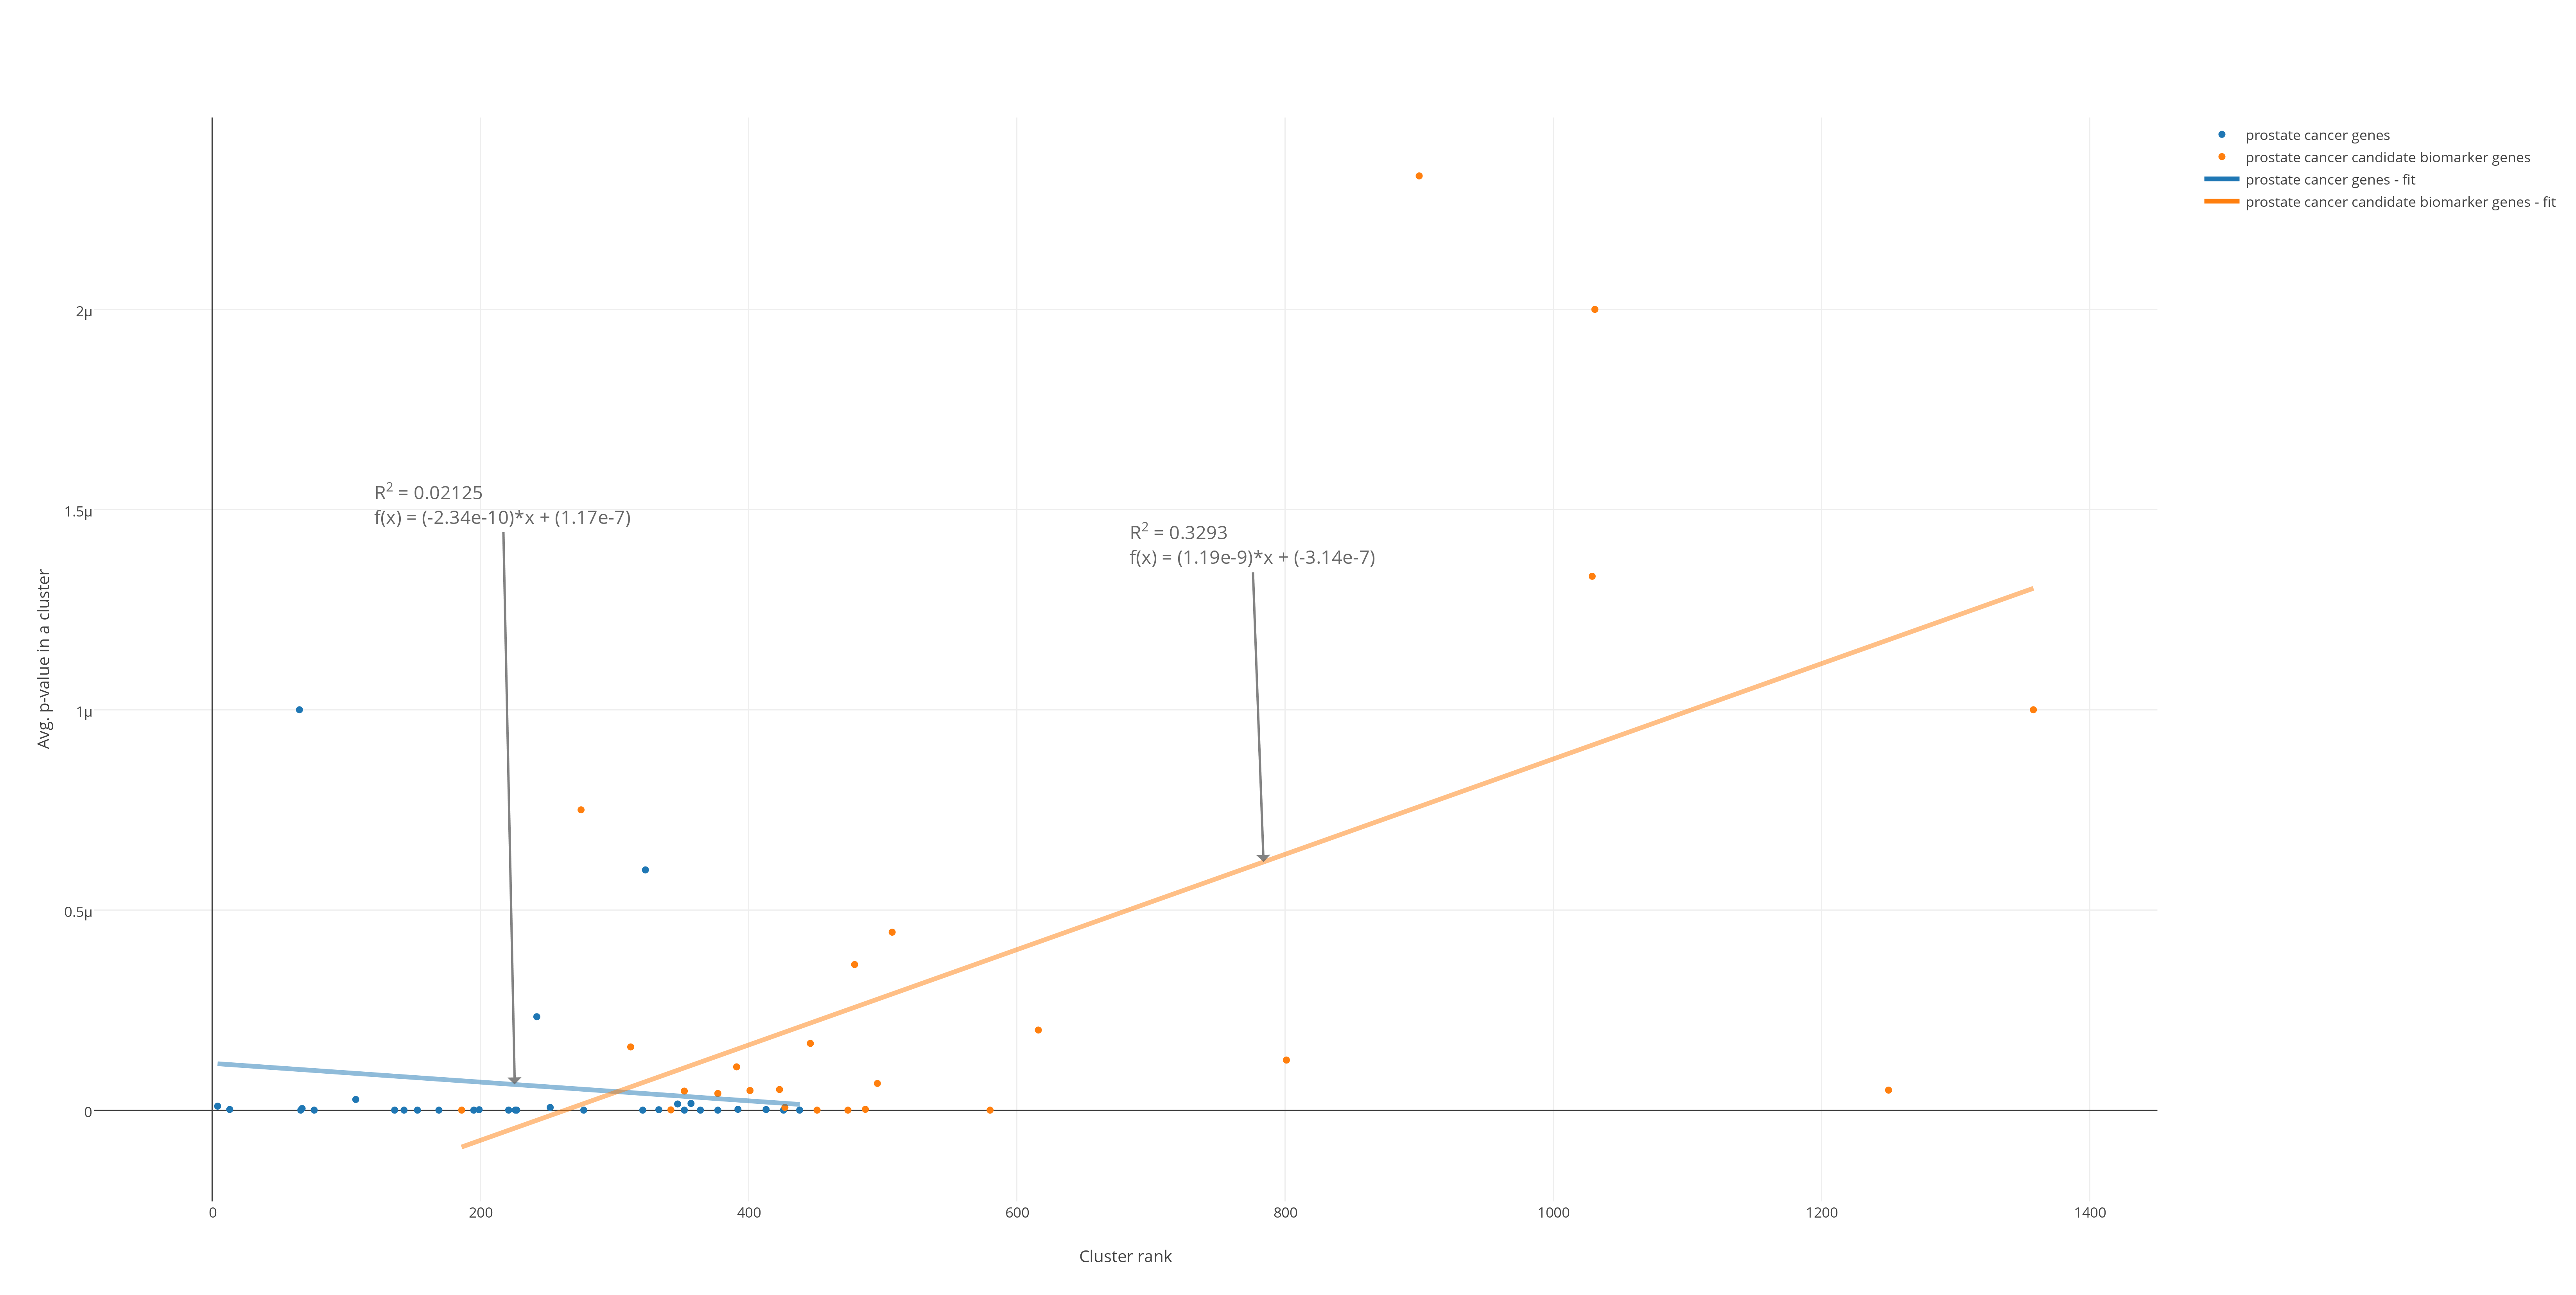
\includegraphics[width=15cm]{maa_experimental_split}
    \caption{Average distribution of p-values in clusters ranked by MAA.}
\end{figure}

\section{Comparison to known biomarkers}
-- Tests from Movember data etc. --

\section{Identification of possible cluster biomarkers}
-- Final list with cluster biomarkers --
